\section{Experimentation Setup}\label{sec:experimentation_setup}
In order to find the best method for learn the Kick Motion, we tested several techniques to compare them and find out that one which converges faster and results in the better and more robust kick. In the next subsections, we will describe each of the methods evaluated in this work.

\subsection{Hybrid Learning Model -- HLM}
In the Hybrid Learning Model (HLM), the training process occurs in two phases. The first one, a supervised learning phase, we learn the keyframe used by using a neural network, reproducing almost the same motion that we already had previously. The intuition behind this is if the agent starts from a good initial point in the optimization problem, it could be easier to get better results applying the gradient in the neighborhood of that point. The reward starts with a good value and the starting motion is well defined. Otherwise, if the optimization starts in a random point, it could be impossible to reach a good motion and probably the agent will get stuck in a local optima. This idea is shown in Figure \ref{optimization_intuition}.

\begin{figure}[!htbp]
	\centering
	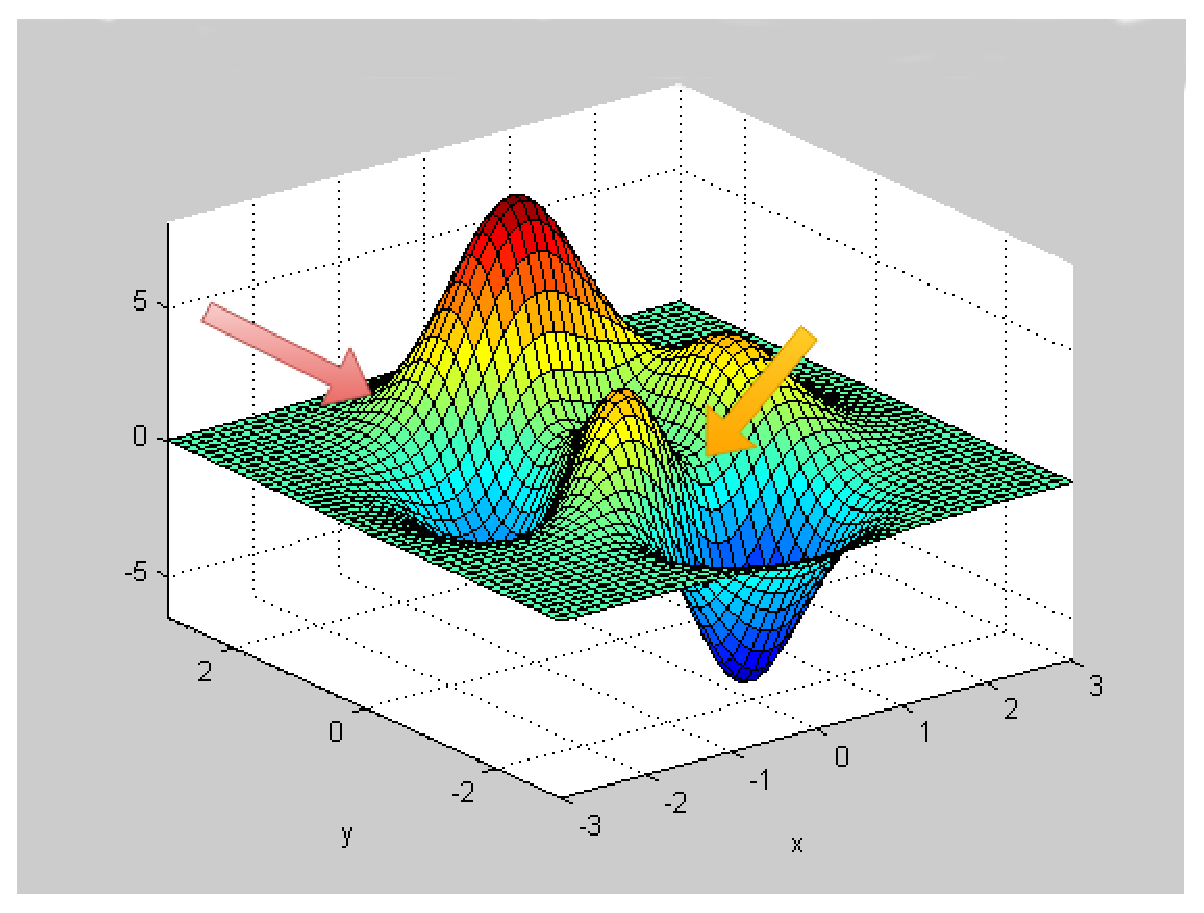
\includegraphics[width=0.5\textwidth]{Cap5/optimization_final.eps}
	\caption{In the hybrid model, we can ensure the starting point is near of the optimal solution (orange arrow); otherwise, the starting point can be bad and harder to optimize (red arrow).}
	\label{optimization_intuition}
\end{figure}

\subsection{Reinforcement with Naive Reward - RNR }
In this learning model, we just use reinforcement learning with a simple and directly reward. As our task is related to kick the ball, the "naive" reward is composed by its velocities after the kick motion, as shown in \ref{naive_reward}, where $s$, $v$ and $u$ are actual state, the vector of velocity and weight parameters, respectively. We call it naive because we don't pass to the learning model any idea of how the motion have to be performed - just what we expect to have as final objective. 

It is important to highlight that the techniques described could be used jointly as building blocks of a more labored model.

\begin{equation}
R(s) = u^{T}v
\label{naive_reward}
\end{equation}

\subsection{Reinforcement with Reference Reward - RRR }
In this learning model we add a term that compares the actual performance with a reference motion, as shown in \ref{complete_reward}:

\begin{equation}
R(s) = w_{ref}^{T}r
\label{complete_reward}
\end{equation}

In this equation, $w_{ref}$ are weight parameters for each joint and $r$ is the absolute value of the difference between joint values in that state and the reference (equation \ref{diffjoints}).

\begin{equation}
r(\theta, \theta_{0}) = \lVert\theta - \theta_{0}\rVert
\label{diffjoints}
\end{equation}

The intuition behind this weight parameters is because we have some joints more important than others. For example, some joints from the leg that kicks the ball themselves could collapse the whole motion if the error is high. On the other hand, joints from the neck are not so important to the kick. Therefore, it's natural to penalize differently in each case.

Lastly, the reference motion used was the keyframe kick previously mentioned and also used in HLM.


\subsection{Reinforcement with Initial State Distribution - RISD}\label{risd}

The Initial State Distribution is a technique related to where the episode starts to collect data to use in the learning. Without this technique, all episodes start in the beginning of the motion. However, the problem of this strategy is because the policy is forced to learn the motion in a sequential manner, first learning the early phases of the motion, and then incrementally progressing towards the later phases. This can be problematic for the kick motion. Another disadvantage of a fixed initial state is the resulting exploration challenge. The policy only receives reward retrospectively, once it has visited a state. Therefore, until a high-reward state has been visited, the policy has no way of learning that this state is favorable \cite{peng2018}.

To implement Initial State Distribution, we used a uniformly random variable that could assume any value in the set of states from the reference motion previously described. Suppose we pick the value $s$. Then, we start the episode running reference motion, from its first state until $s$. Finally, we start to collect data and perform the actions from the running policy.

\subsection{Reinforcement with Early Termination - RET}

The Early Termination technique is related to where the episode ends. Without early termination, all motions stops in the same state, which means that the episode length is fixed. The problem of this is because if the motion fails somehow during its execution, all the data collected after the failure will harm learning and evaluation of later stages.

In the kick motion task, the early termination will be triggered when the robot falls during the motion. This behavior will ensure two things: first, that we don't collect wrong data, as mentioned before; and second, to gain more reward and have longer episodes, the agent will be forced to learn a kick motion that doesn't fall -- which will be very good in game situation.



\section{Supervised Learning Setup}\label{supervised_learning_setup}
\subsection{The Dataset}\label{AA}
In order to use supervised learning for learning keyframe motions using neural networks in the HLM model, we first need to construct a dataset. A dataset consists of samples of keyframe steps. Samples were collected within the Soccer 3D environment with a frequency of 50 Hz. We acquired these samples in two different ways.

In the first one, we commanded an agent of our team to execute specific motions and sampled the reference joint positions computed by our code. In this case, we sampled the kick and get up keyframe motions \cite{muniz2016}. Notice that, for this approach to be successful, one needs access to the source-code.

The second approach involved changing the Soccer 3D server source-code to provide current joint positions of a given robot, in a similar way as described in \cite{macalpine2013}. This allowed us to acquire motion datasets from other teams, without any knowledge of how these movements are implemented. In this case, we collected two types of kicks based on keyframes and sampled joint values of the walking engine \cite{AAAI12-MacAlpine}.


\subsection{Neural Network Architecture and Hyperparameters}

The neural network has to be able to learn how to interpolate between samples, which actually happens. The architecture that performed best -- in terms of mean absolute error minimization and simplicity -- is shown in Figure ~\ref{fig:model_plot}. A deep neural network with 2 hidden, fully connected layers of 75 and 50 neurons was used. The output layer has 23 regression neurons, which represent the 22 joint angles and a neuron which output indicates if the motion has ended or not. The neurons in each hidden layer use the LeakyReLU activation function \cite{leakyrelu}: 

\[
  f(x) = \left\{
     \begin{array}{@{}l@{\thinspace}l}
       \alpha x,   & \quad x < 0  \\
       x, & \quad x \ge0 \\
     \end{array}
   \right.
\]
where $\alpha$ is a small constant. This activation function was used to improve the representation capacity of the neural network, adding support for non-linear functions.

\begin{figure}[!htbp]
\centering
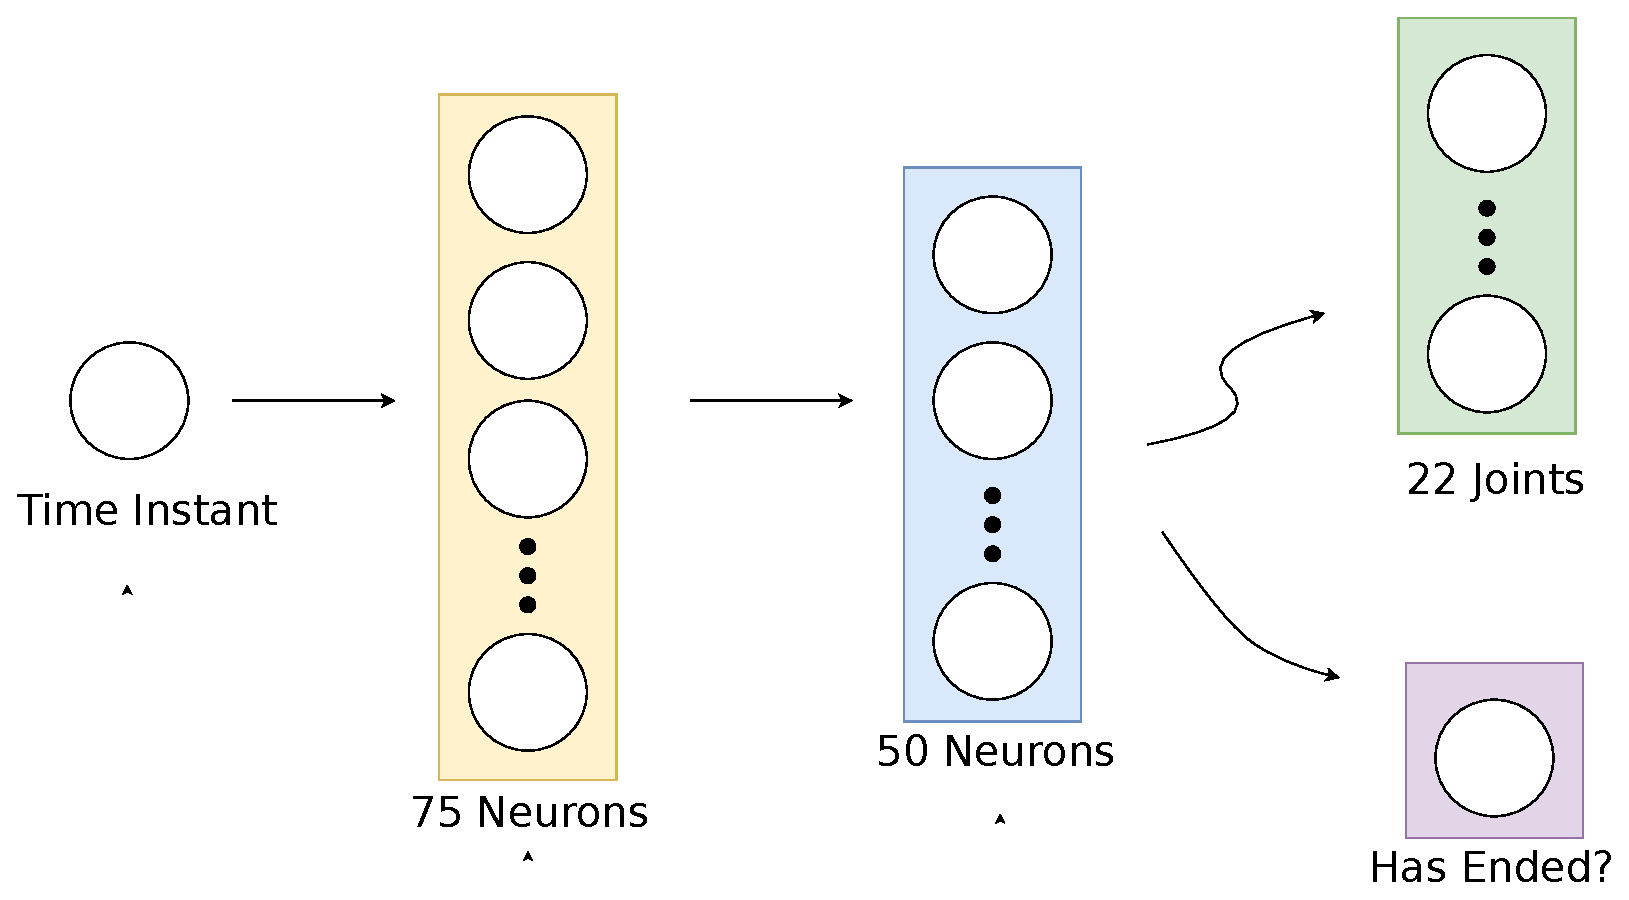
\includegraphics[width=0.5\textwidth]{Cap5/architecture}
\caption{The architecture of a neural network designed to learn motions.}
\label{fig:model_plot}
\end{figure}

This architecture resulted in thousand of parameters to optimize, as exposed in Table \ref{tab:network_summary}. A very high number, when compared to more traditional optimization approaches \cite{AAAI12-MacAlpine}. Notice that, by increasing the number of parameters usually allows representing better movements.

\begin{table}[htbp]
\caption{The Network Summary}
\begin{center}
\begin{tabular}{|c|c|c|c|}
\hline
\textbf{Layer}&{\textbf{Neurons}}& \textbf{Activation}& \textbf{Parameters} \\
\hline
Dense & 75 & LeakyReLU & 150  \\
\hline
Dense & 50 & LeakyReLU & 3800 \\
\hline
Dense & 23 & Linear & 1173 \\
\hline
\end{tabular}
\begin{tabular}{|c|c|}
\hline
\textbf{Total Parameters} & 5123 \\
\hline
\end{tabular}
\label{tab:network_summary}
\end{center}
\end{table}


\subsection{The Training Procedure}
Since keyframe motions are executed in an open-loop fashion, the sequence of joint positions are always the same for different repetitions, independently of robot's state. Therefore, by adding samples of multiple executions of the same motion would not make our dataset richer. So, we decided to use only one repetition for each movement for faster training. In the case of the walking motion, we collected samples within one walking period.

During the training, we used 50 thousands epochs divided into 5 training phases, where the learning rate was decreased between phases, in order to achieve better performance. First, we executed 30000 epochs, by using the learning rate of 0.001. The other phases had 5000 epochs each, and we decreased the learning rate by 0.0002 in each phase.

Furthermore, we used Adam optimization \cite{adam2014}, during the whole training. The loss function used was the mean squared error, as explained in Subsec. \ref{sec:neural_networks}. We decided this loss function is adequate for this problem, mainly because it strongly penalizes large errors, which can collapse the whole motion.

\subsection{The Deployment in the Soccer 3D Environment}
In order to perform the network design and the training procedure, we used the Keras \cite{chollet2015keras} framework coupled with Tensorflow \cite{tensorflow2015-whitepaper} as backend. After training, the weights were frozen and converted to a specific format, which was readable, by using the Tensorflow C++ API integrated within agent's code. Hence, the training was performed outside the environment, but the agent actually has computed network inferences, during the simulation execution.

\section{Reinforcement Learning Setup}

To use a Reinforcement Learning model, we need to define a policy representation and a task which the agent will follow during the process.

\subsection{Policy Representation}

The policy is represented by a neural network similar to the supervised learning model. A state is described as the stage of kick motion. An action is a set of joint values that has to be applied by the agent in that state.

In HLM, the architecture from both value function and policy networks is that described by section \ref{supervised_learning_setup}. On the other cases, the network is composed by three building blocks: an input normalization Filter, the neural networks themselves and a Gaussian action space noise.

\subsubsection{Input Normalization Filter}\label{sec:inputnorm}
The input normalization filter, also know as feature scaling, has the objective of normalize the input to avoid the problem of vanishing and exploding gradients by applying updates through all dimensions in equal proportions, as illustrated in Figure \ref{inputnormfig}. This normalization happens at each pass in the network, re-calculating mean and standard deviation using the new examples. Hence, this method helps during the convergence.

\begin{figure}[!htbp]
	\centering
	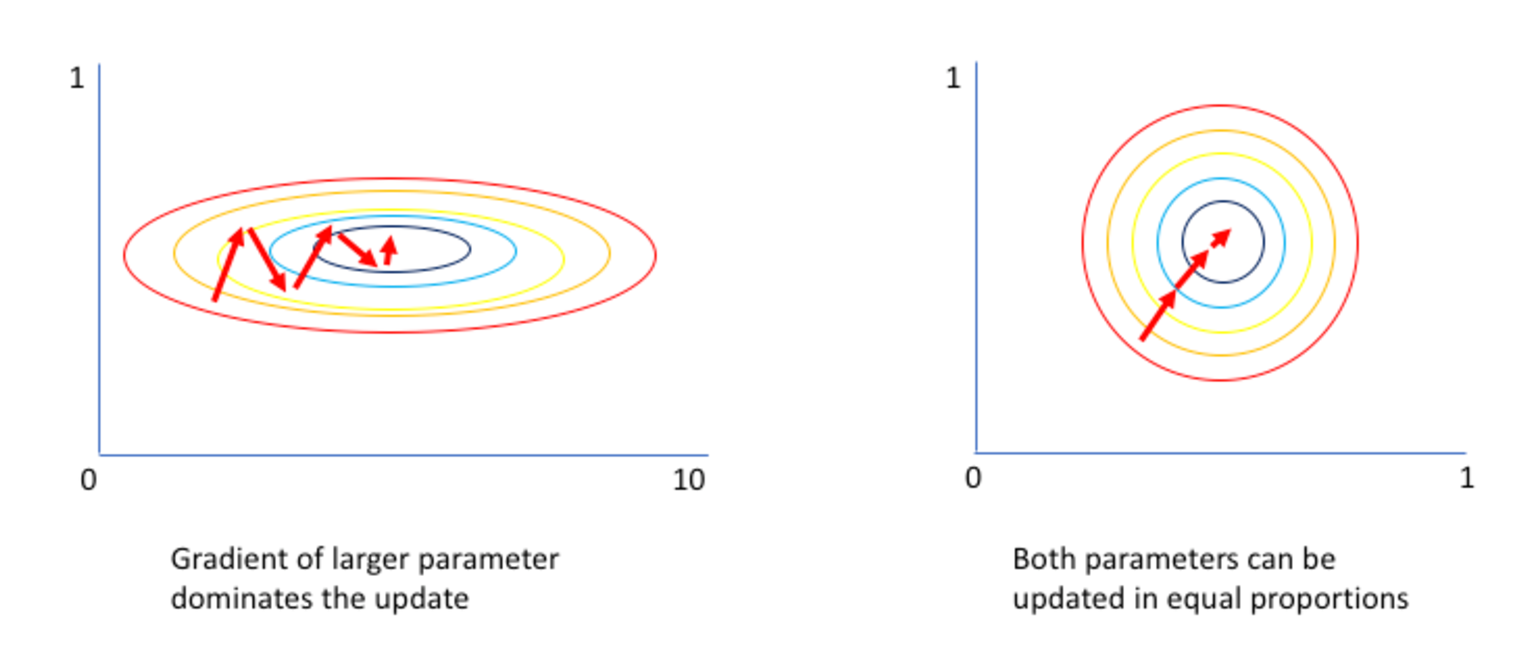
\includegraphics[width=0.5\textwidth]{Cap5/inputnorm.eps}
	\caption{Intuition behind input normalization}
	\label{inputnormfig}
\end{figure}

\subsubsection{Neural Network}
As an actor-critic model, we have two networks: one for the value function and other for the policy itself. They have the same architecture: two layer, fully connected, with 64 neurons in each hidden layer and hyperbolic tangent as activation function. The architecture is illustrated in Figure \ref{rlnetwork}. Table \ref{tab:rl_network_summary} summarizes the parameters in this new architecture, also considering the parameters from the Gaussian Action Space Noise, described in \ref{gasp}.

\begin{figure}[!htbp]
	\centering
	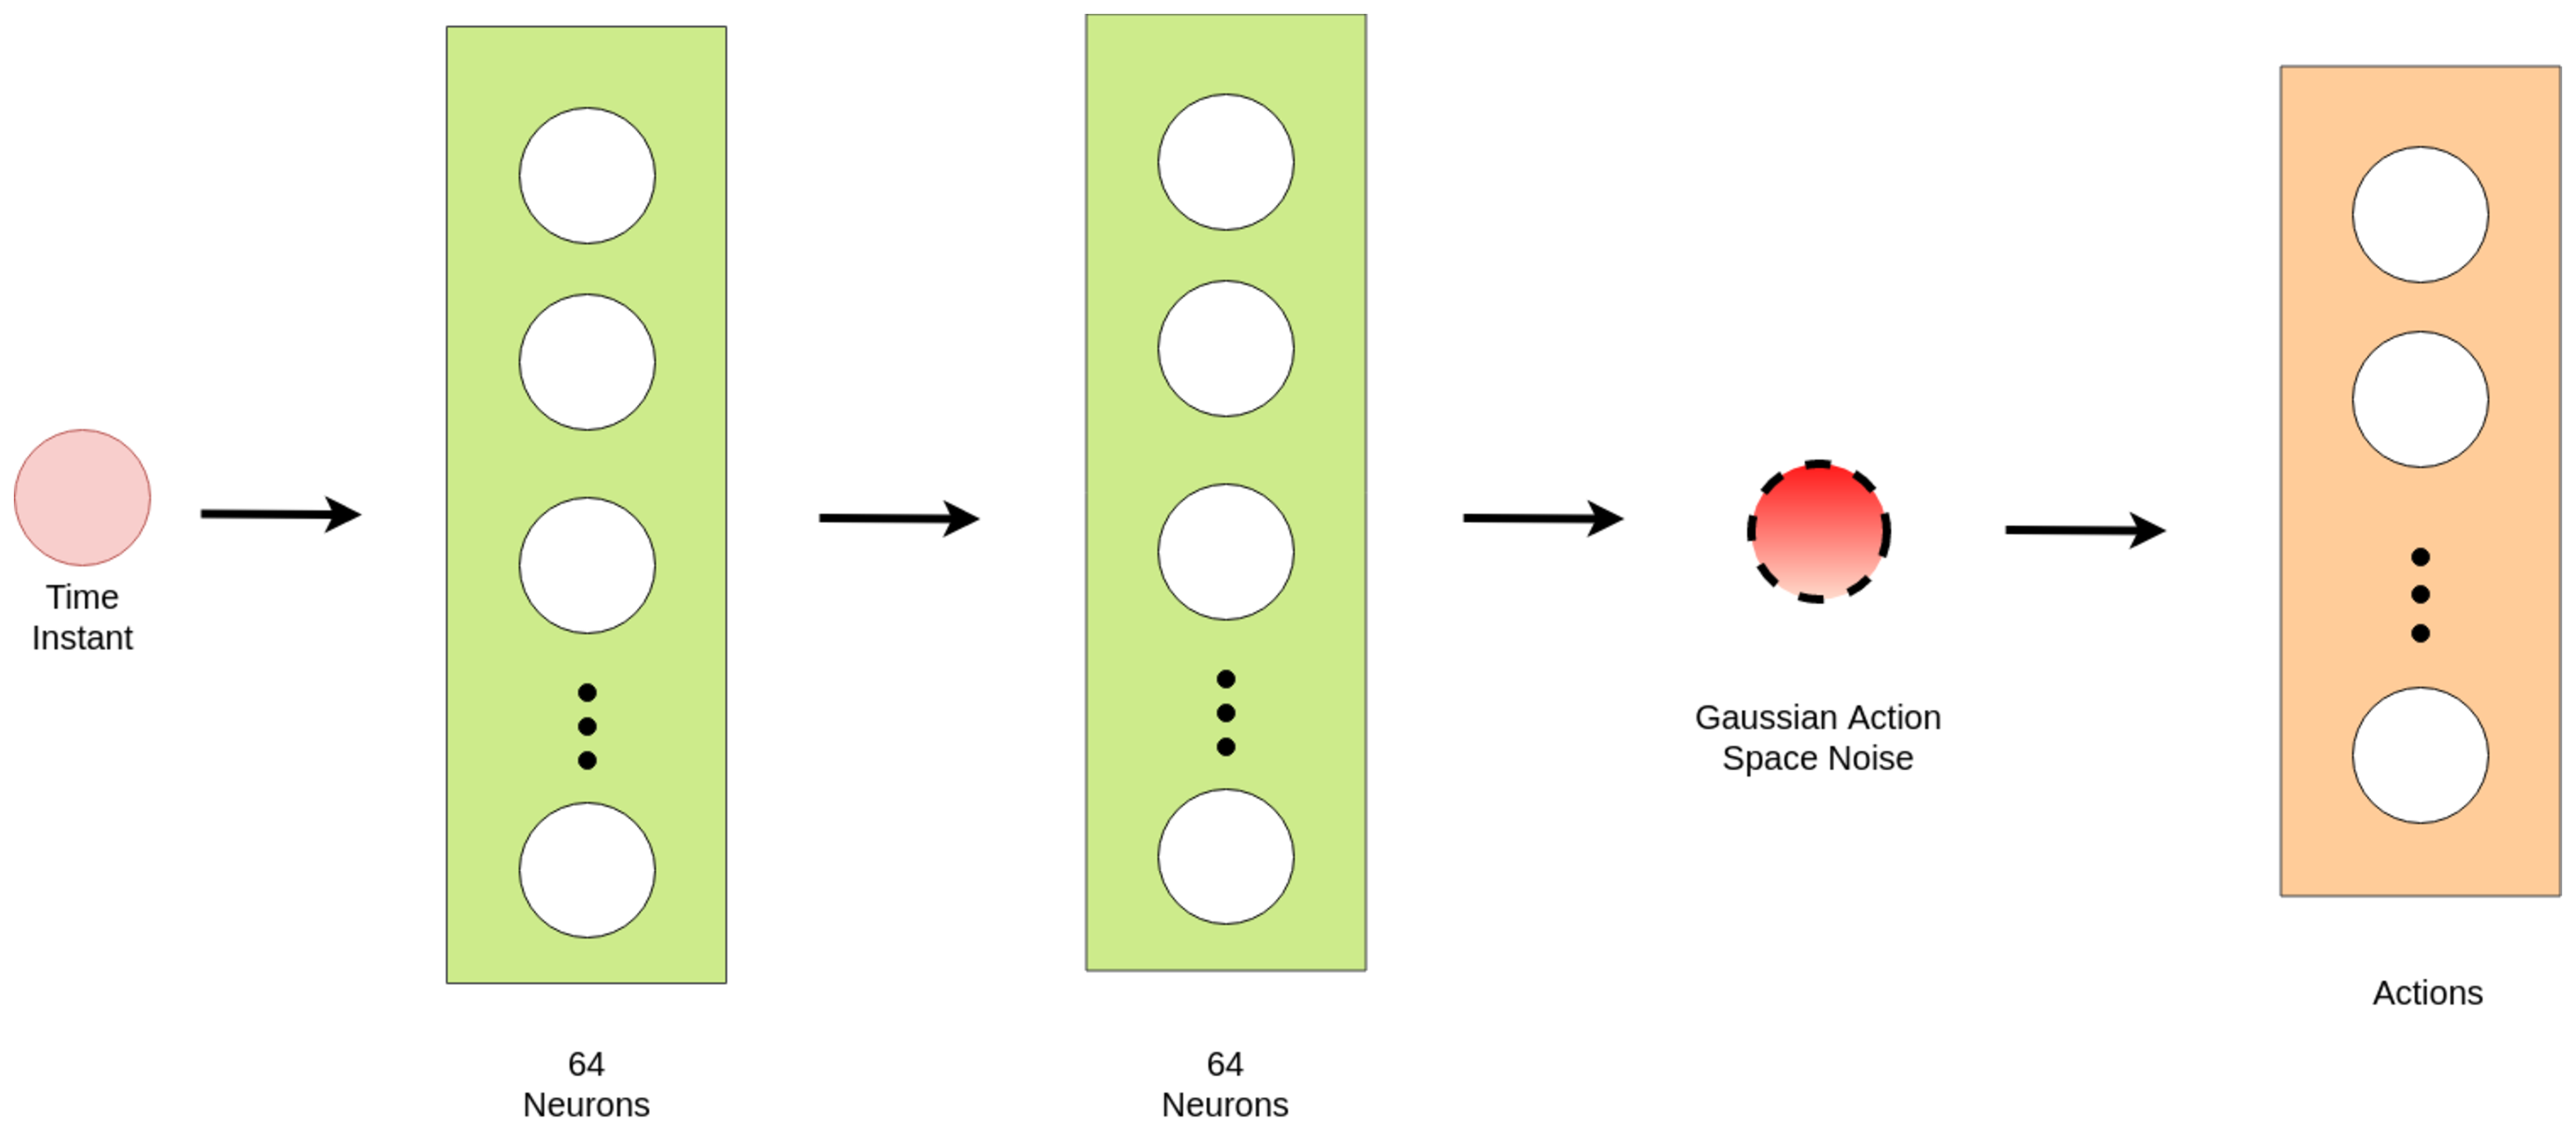
\includegraphics[width=0.5\textwidth]{Cap5/rlnetwork.eps}
	\caption{Architecture used by pure Reinforcement Learning models.}
	\label{rlnetwork}
\end{figure}

\begin{table}[htbp]
	\caption{The Reinforcement Learning Network Summary}
	\begin{center}
		\begin{tabular}{|c|c|c|c|}
			\hline
			\textbf{Layer}&{\textbf{Neurons}}& \textbf{Activation}& \textbf{Parameters} \\
			\hline
			Dense & 64 & $tanh$ & 128  \\
			\hline
			Dense & 64 & $tanh$ & 4160 \\
			\hline
			Output & 23 & Linear & 1495 \\
			\hline
			Noise & 23 & Linear & 23 \\
			\hline
		\end{tabular}
		\begin{tabular}{|c|c|}
			\hline
			\textbf{Total Parameters} & 5806 \\
			\hline
		\end{tabular}
		\label{tab:rl_network_summary}
	\end{center}
\end{table}


\subsubsection{Gaussian Action Space Noise}\label{gasp}

The last idea explored in this policy representation is the Gaussian action space noise for better exploration. It adds adaptive noise to the action space of the neural network. Discrete RL uses $\epsilon$-greedy \cite{Watkins:1989} to confer exploration. Gaussian action space noise injects normal randomness directly into the actions of the agent, altering the types of decisions it makes and helping algorithms explore continuous environments more effectively. The Figure \ref{gaussiannoise} illustrates this technique.


\begin{figure}[!htbp]
	\centering
	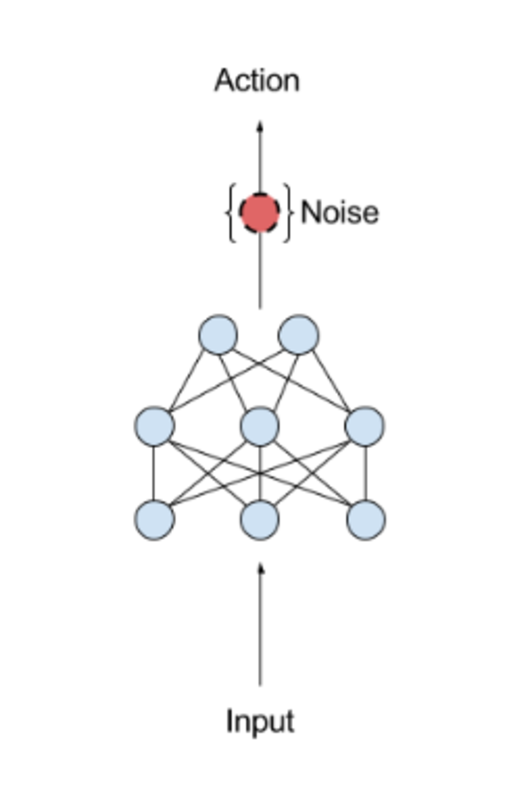
\includegraphics[width=0.3\textwidth]{Cap5/gaussiannoise.eps}
	\caption{Gaussian noise applied to action space to ensure better exploration in continuous environments.
	\cite{parameternoiseblog}
	}
	\label{gaussiannoise}
\end{figure}

\subsection{Task Description}
The learning task consists in the activity the agent will execute in order to achieve the expected behavior through the policy. In this experimentation, we would like to learn the kick motion. Therefore, is straightforward that the scenario is based on kick the ball.

The agent is started in a fixed position of the soccer field. The ball, on the other hand, starts in a position $\alpha_{ball}$ meters from the agent, in front of him. The parameter $\alpha_{ball}$ can be optimized in order to decide the best position the agent have to stop to kick the ball better. However, for this experimentation, we fixed its value.

We repeat the following flow: in the beginning of the episode, all the joints are initialized in a certain value that correspond to the joints the robot assume when it stops to walk and will start the kick motion. Then, we start the learning steps, applying the joints from the neural network to the robot. When we use RISD, there's a intermediate phase executing the reference motion, as described in \ref{risd}.

After the execution of those steps, we finalize the episode turning all the joints to zero. When there's no Early Termination, this happens after a fixed number of steps that we can ensure the motion has over. Otherwise, this occurs when the early termination condition is reached.

Figure \ref{taskdescription} shows the initial setup from the task.


\begin{figure}[!htbp]
	\centering
	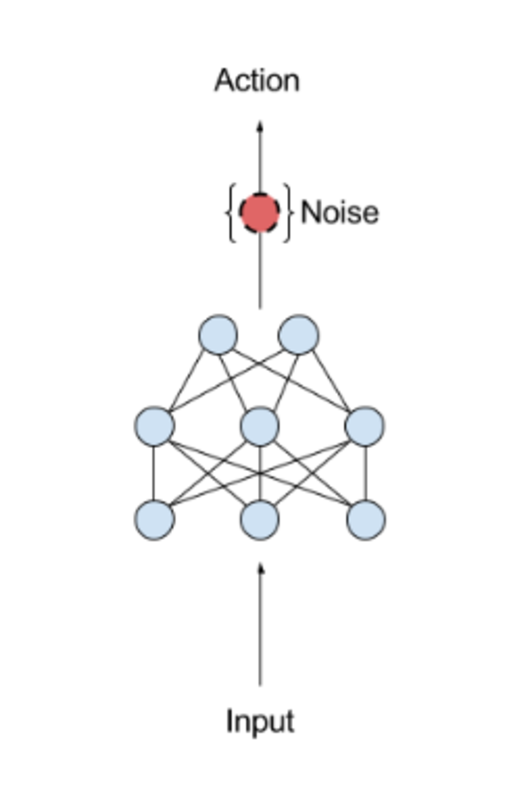
\includegraphics[width=0.3\textwidth]{Cap5/gaussiannoise.eps}
	\caption{Initial setup from the task used to learning kick motion.}
	\label{taskdescription}
\end{figure}

\section{Infrastructure}
\subsection{Reinforcement Learning Server}\label{rlarchitecture}

Figure \ref{rlserver} shows the architecture used to integrate the learning algorithm, agent and simulation environment. The simulation server exposes a state to the soccer agent, which model this information and passes to the learning algorithm that chooses a action accordingly and returns to the agent. Then, it applies this action in the environment, modifying its state, completing the cycle.

\begin{figure}[!htbp]
	\centering
	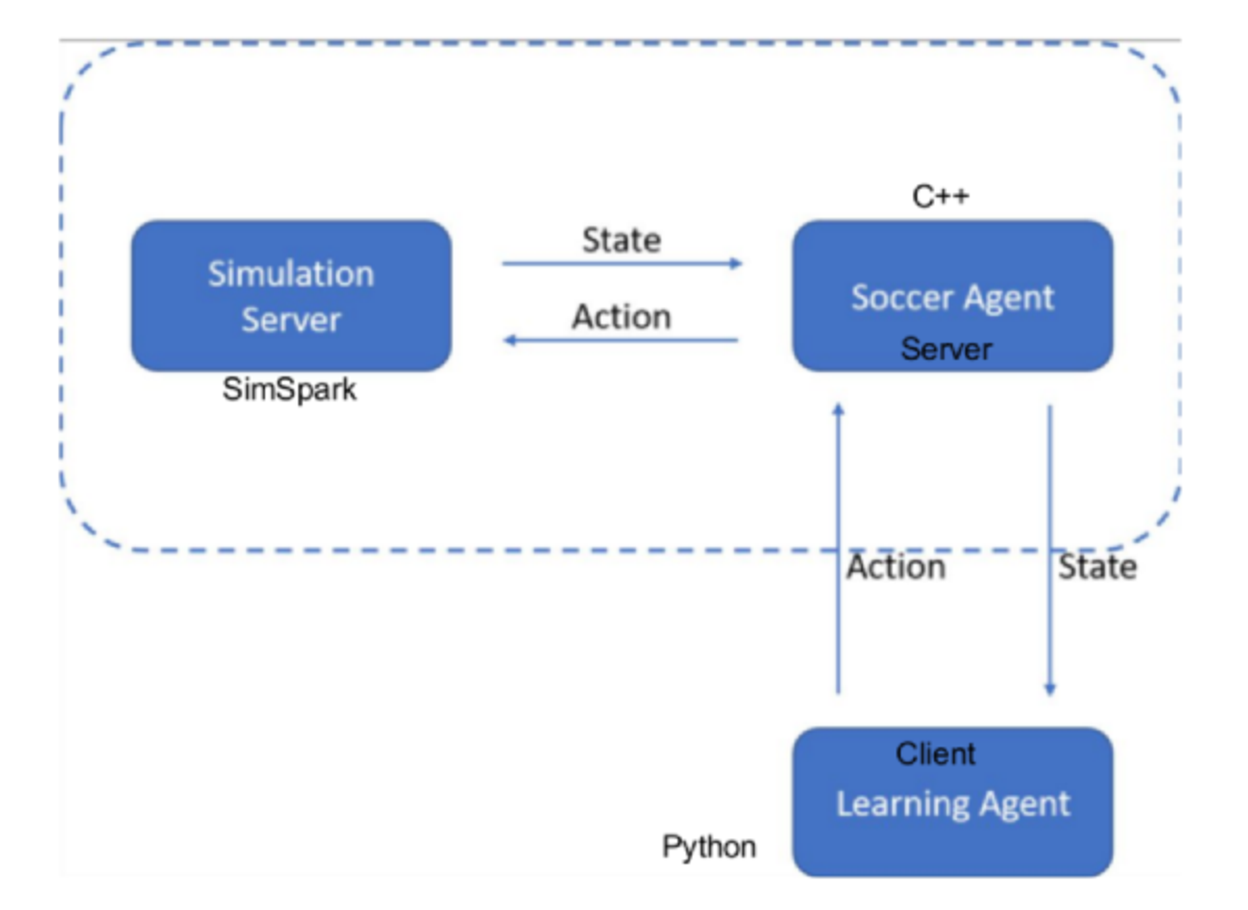
\includegraphics[width=0.3\textwidth]{Cap5/rlserver.eps}
	\caption{Reinforcement Learning Server Architecture.
		\cite{tgmuzio}
	}
	\label{rlserver}
\end{figure}

\subsubsection{Simulation Server}

The simulation environment used, as mentioned before, is Simpark. It uses a TCP Socket to communicate with the agent and exposes a interface for querying the ground truth state for many features from the agent - which can be helpful to state evaluation and avoids to use agent's perceived data that has noise. 

\subsubsection{Soccer Agent}
The agent used is from ITAndroids Soccer 3D team and it leads with the perception information sent from the server, model the world with this information and make decisions accordingly. Additionally, there's a entity, called Wizard, whose purpose is query the ground truth state. All this code is written in C++ and the task described in \ref{taskdescription} was implemented in the agent itself.

Other tool that worth mention is RoboViz, a publicly available visualization tool that allows a few improvements over the default visualization tool. We used it to verify if the task was implemented successfully.

\subsubsection{Learning Agent}\label{learningagent}

We created another interface to integrate the Soccer Agent with the algorithms used in this experimentation. These were implemented by OpenAI Baselines \cite{baselines}, a repository of high-quality implementations of reinforcement learning algorithms whose purpose is make easier for the research community to replicate, refine, and identify new ideas, and create good baselines to build research on top of. The community developed those algorithms using Python language with the Tensorflow \cite{tensorflow2015-whitepaper} framework.

This integration was done using gRPC \cite{grpc}, an open source remote procedure call (RPC) system that generates cross-platform client and server bindings. It uses HTTP/2 for transport and Protocol Buffers \cite{protocolbuffers} as the interface description language, serializing structured data.




\subsection{Neural Network Deployment}

When we use the architecture from \ref{rlarchitecture}, two problems related to the neural network deployment arise.

The first one is related to the HLM. We have a supervised learning model trained using the framework Keras outside the environment and with no relation to OpenAI Baselines. Therefore, we need a way to import this model from Keras model into the learning algorithms.

The second problem is to deploy the network from learning algorithm to the soccer agent. When the network is trained using OpenAI Baselines, there's no contact between the soccer agent and the model. As described in \ref{learningagent}, there's a interface to communicate the actions between them. All calculations happens in only one side. However, during a game, it's not possible to maintain this dependency, so we need a way to run the network inside soccer agent and without the whole training structure.

\subsubsection{Import Supervised Model into OpenAI Baselines}

To solve this problem, it's important to understand how Keras works and what's the challenge behind this import. 

Keras works on top of lower level machine learning frameworks. Its purpose is make easier to prototype and train models with few lines of code. With Keras, developers don't need to understand in deep how computational graphs works and some math behind the models. Actually, this framework wraps code from the lower level ones. Therefore, even being easier to use, all the computation and data structures remains the same.

As back-end framework that Keras runs on top of, we used Tensorflow. As described previously, it creates a computational graph with math tensors as inputs that "flow" inside and returns the expected result.

Given that context, the idea is straightforward: we create a "Kick Policy" class, that creates the model using Keras, load its weights, gets the output tensor and injects in the rest of Tensorflow's computational graph related to the learning algorithm. The Algorithm \ref{importnetworkpseudocode} explains sequentially this idea.

\begin{algorithm}
	\caption{Import Keras model into Tensorflow}
	\begin{algorithmic} 
		\REQUIRE Keras output model
		\STATE $model \leftarrow createKerasModelStructure()$
		\STATE $model.load\_weights(keras\_output\_model)$
		\STATE $outputTensor \leftarrow model.output$
		\STATE Inject $outputTensor$ in the rest of computational graph
	\end{algorithmic}
	\label{importnetworkpseudocode}
\end{algorithm}

It's important to mention that the $load\_weights$ operation already initializes the graph variables and if we initialize them again, we lose the pre-trained weights.

The biggest problem of this integration is we can't use Input Normalization Filter and Gaussian Action Space Noise, described in \ref{sec:inputnorm} and \ref{gasp}, respectively. Therefore, we can face gradient and exploration problems during learning.

\subsubsection{Export OpenAI Baselines onto Soccer Agent}

As mentioned earlier, Tensorflow creates a data flow graph with all operations executed during the algorithm. Figure \ref{fig:dataflowgraph} shows the whole graph for PPO used in this experimentation. However, we need to export only the policy network itself.

\begin{figure}[!htbp]
	\centering
	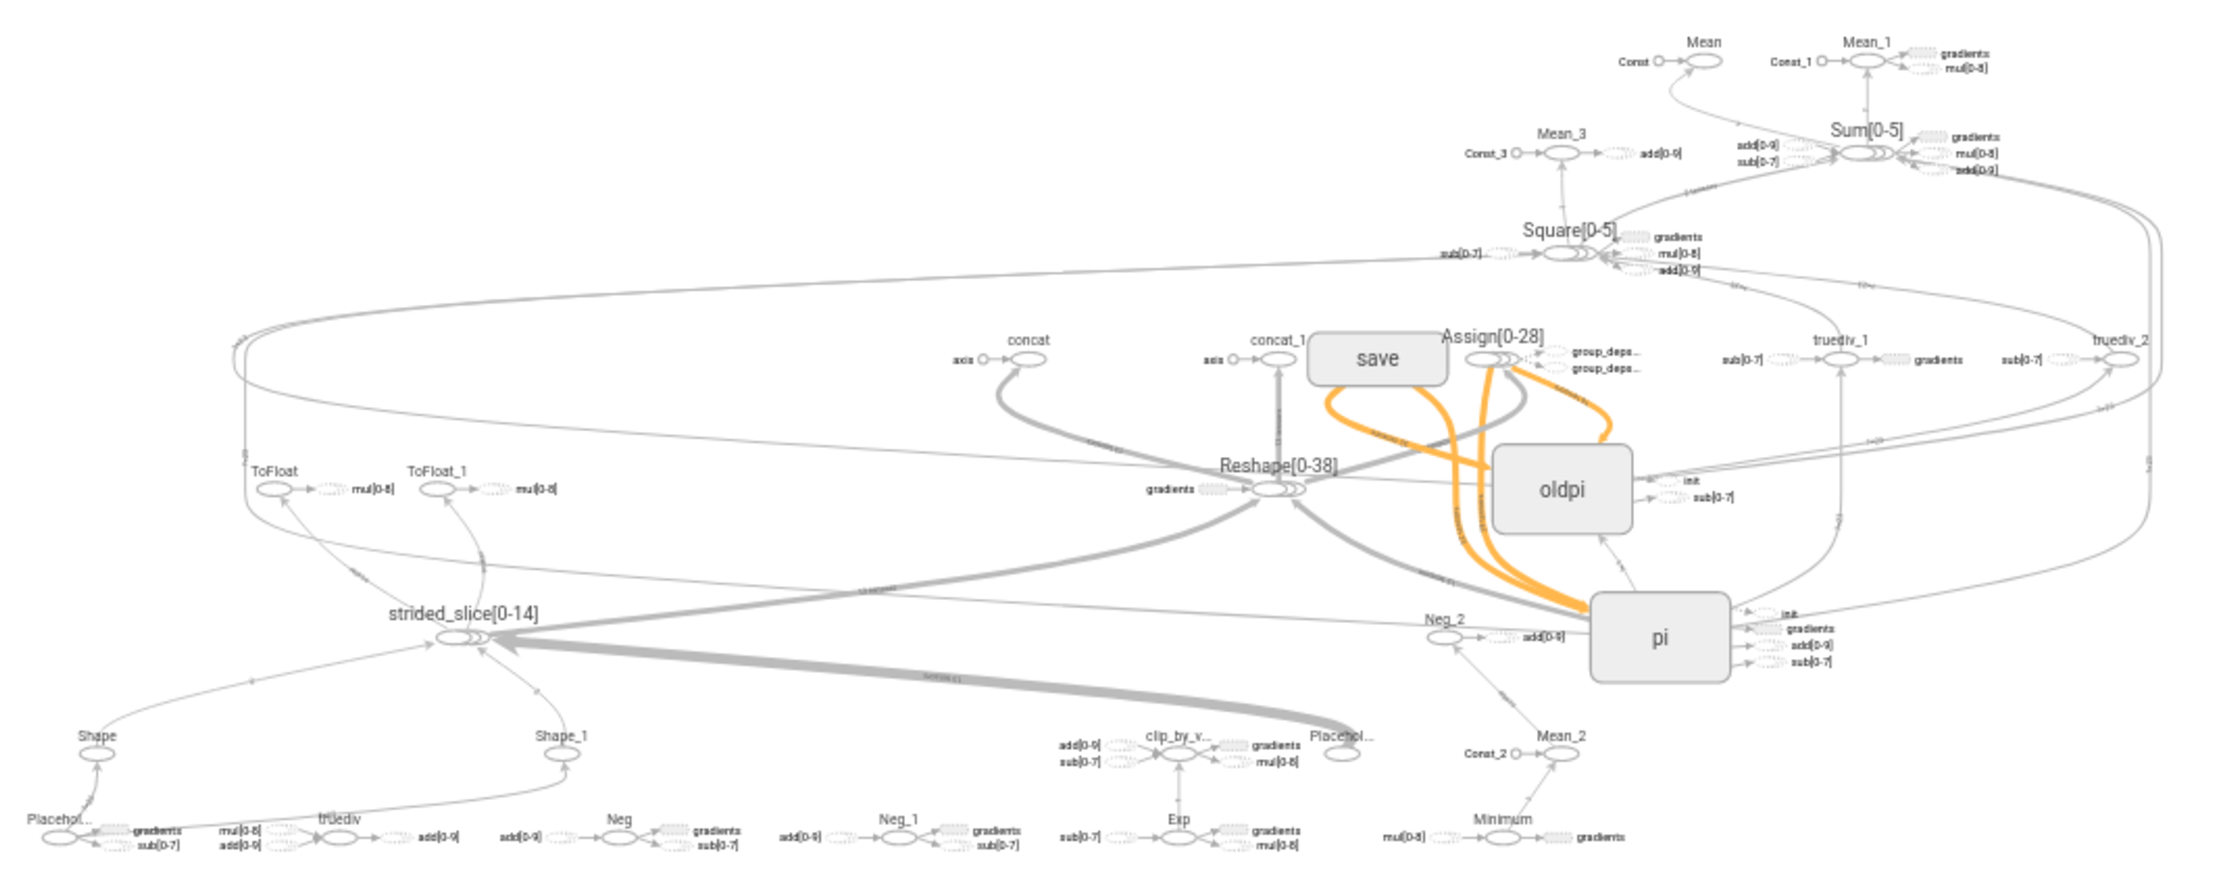
\includegraphics[width=1.1\textwidth]{Cap5/dataflowgraph.eps}
	\caption{Data flow graph for PPO algorithm.
	}
	\label{fig:dataflowgraph}
\end{figure}

It is important to mention that ``policy network" mean only the neural network that maps state to actions, and not the whole policy node ``pi" in Figure \ref{fig:dataflowgraph}. The ``pi" node also have the value function network and gaussian noise in action space, only needed during the learning process. Figure \ref{fig:pigraph} shows the whole ``pi" node.

\begin{figure}[!htbp]
	\centering
	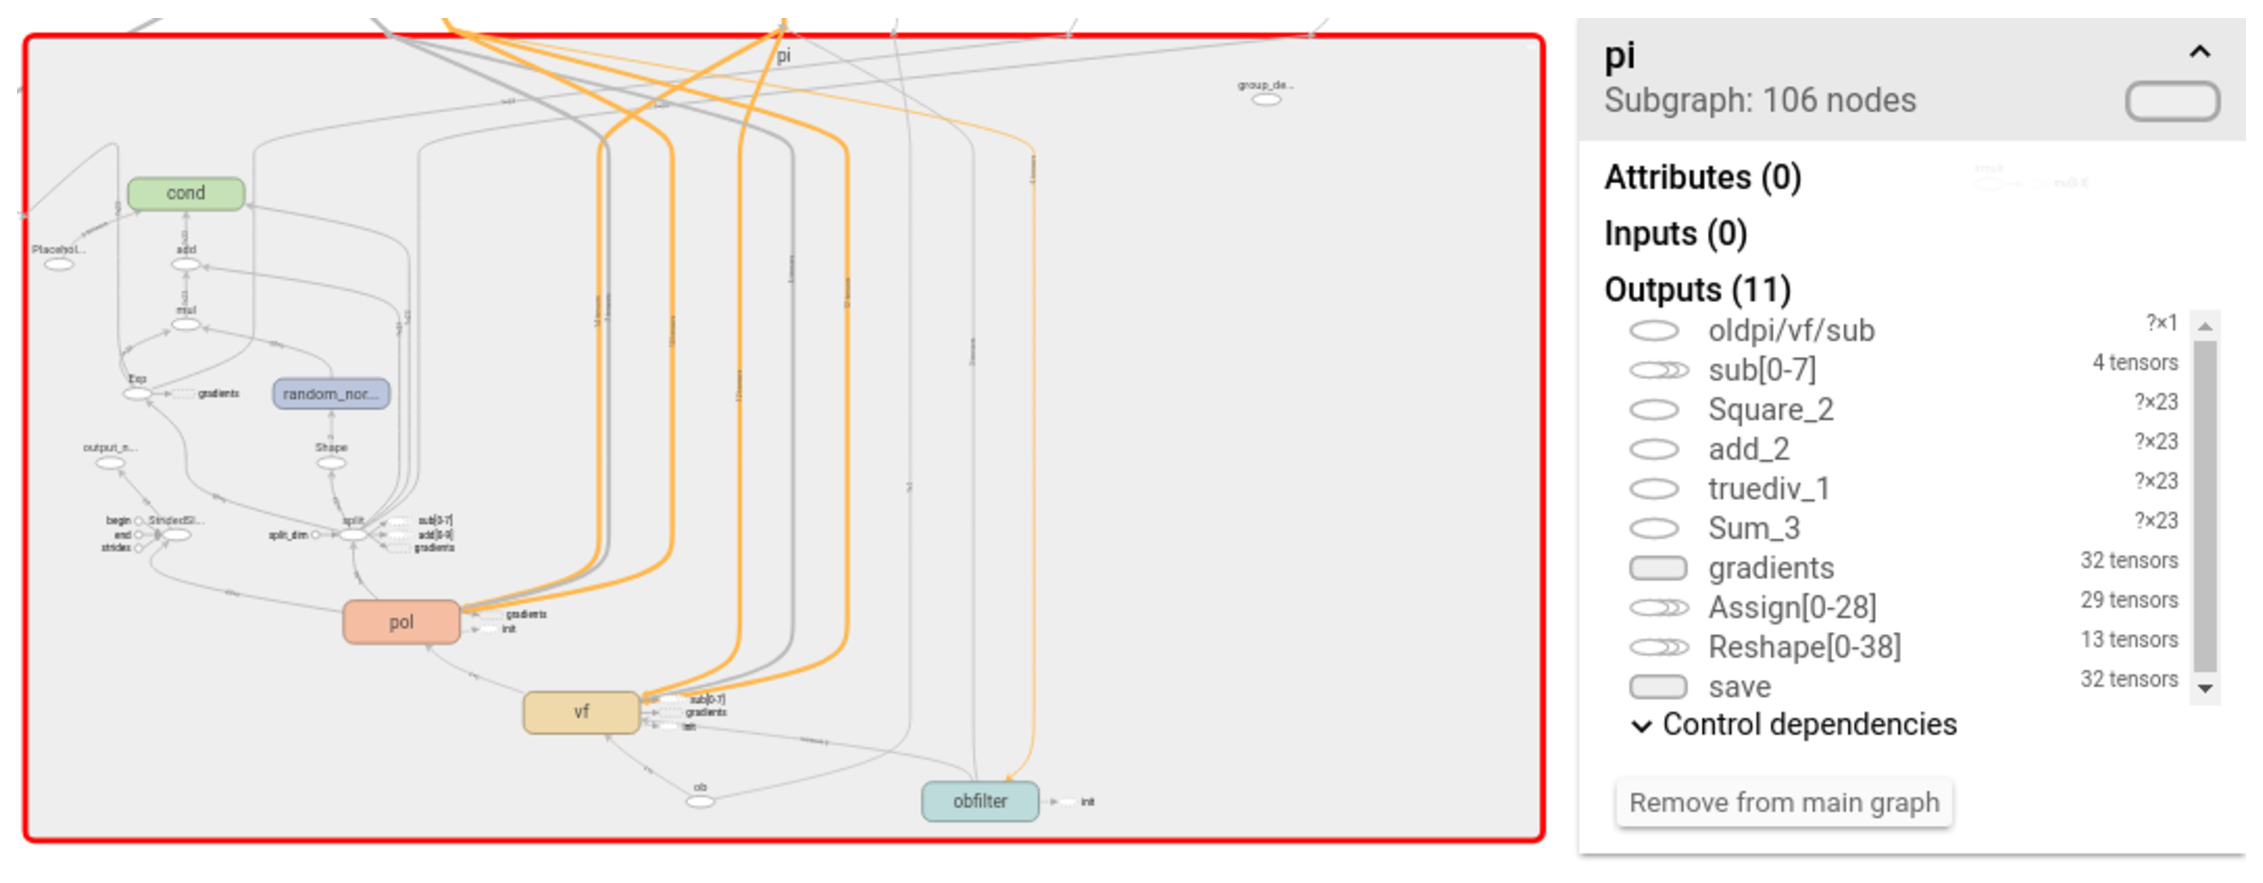
\includegraphics[width=1.1\textwidth]{Cap5/pigraph.eps}
	\caption{ ``Pi" data flow node from PPO.
	}
	\label{fig:pigraph}
\end{figure}

Therefore, to export this policy network, we need to add a new "identity" node in the output from that. This node has the same resultant tensor, but it is possible to label it and we can freeze the subgraph whose output is the labeled node itself. Internally, Tensorflow will start freezing the output node and its dependencies, recursing until input nodes. Then, we save this data structure in a proto file that we read using the C++ API in the soccer agent. Figure \ref{fig:policygraph1} and \ref{fig:policygraph2} show the policy data flow graphs from Figures \ref{rlnetwork} and \ref{fig:model_plot}, respectively.



\begin{figure}[!htbp]
	\centering
	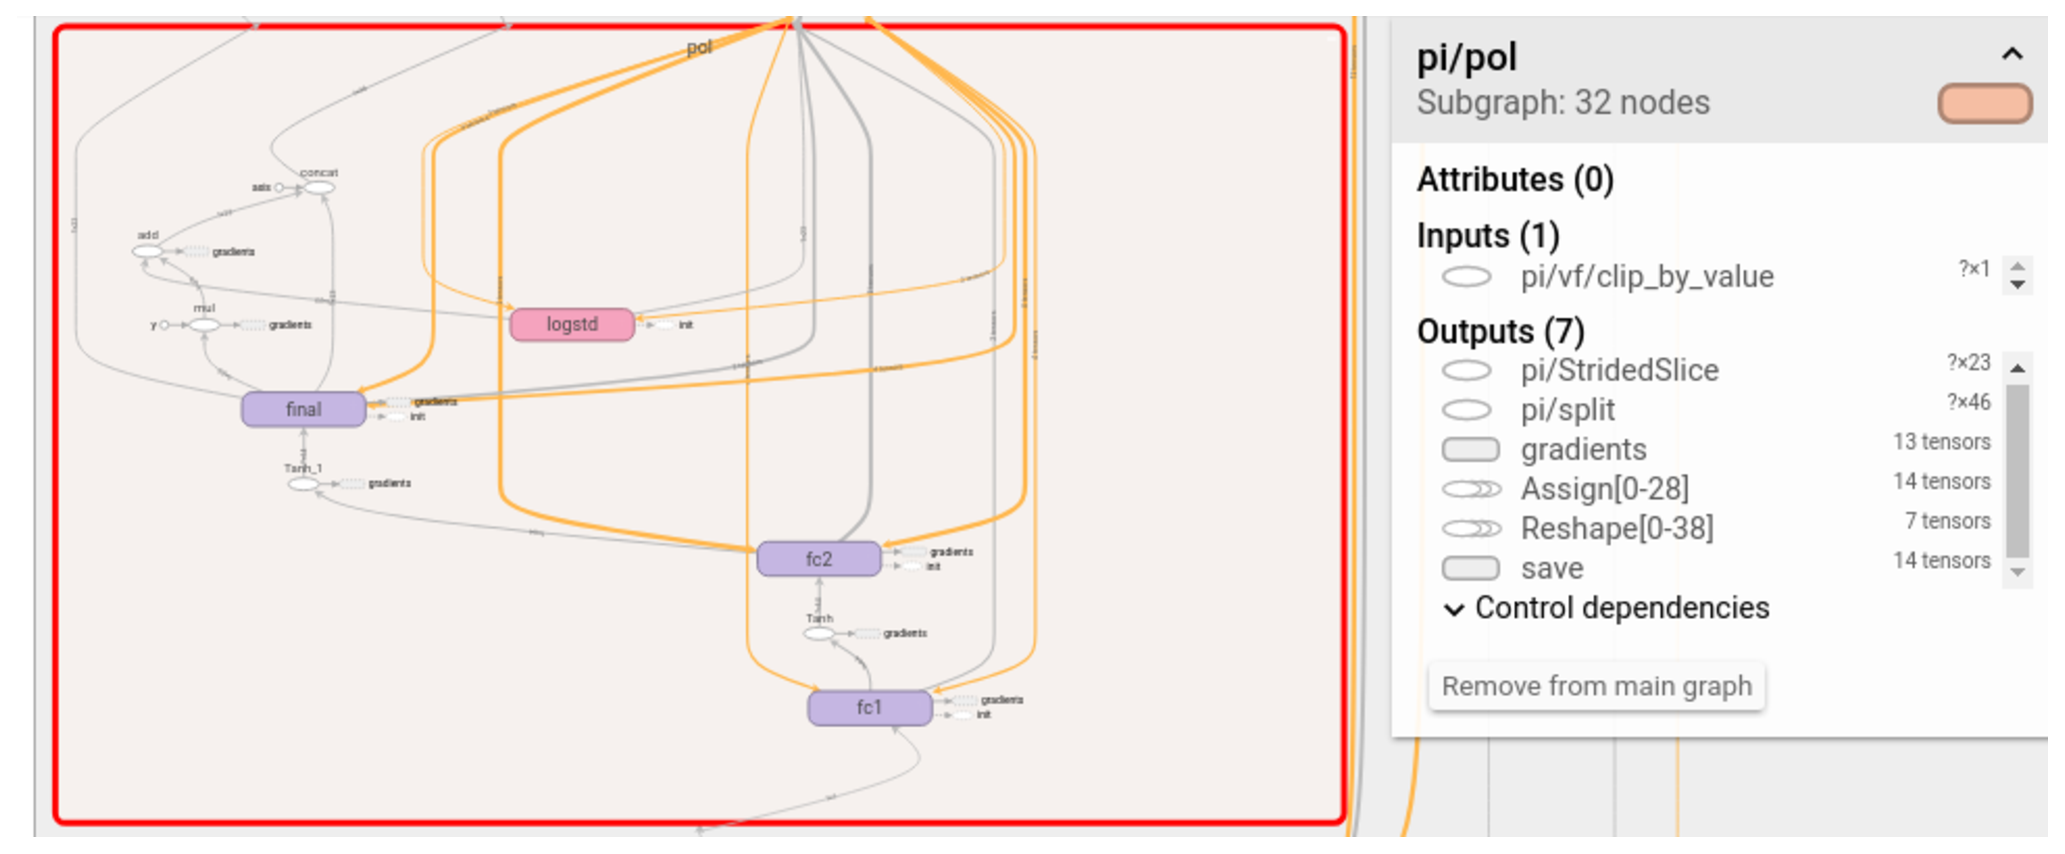
\includegraphics[width=1.1\textwidth]{Cap5/policygraph1.eps}
	\caption{ Policy data flow graph from Figure \ref{rlnetwork}
	}
	\label{fig:policygraph1}
\end{figure}

\begin{figure}[!htbp]
	\centering
	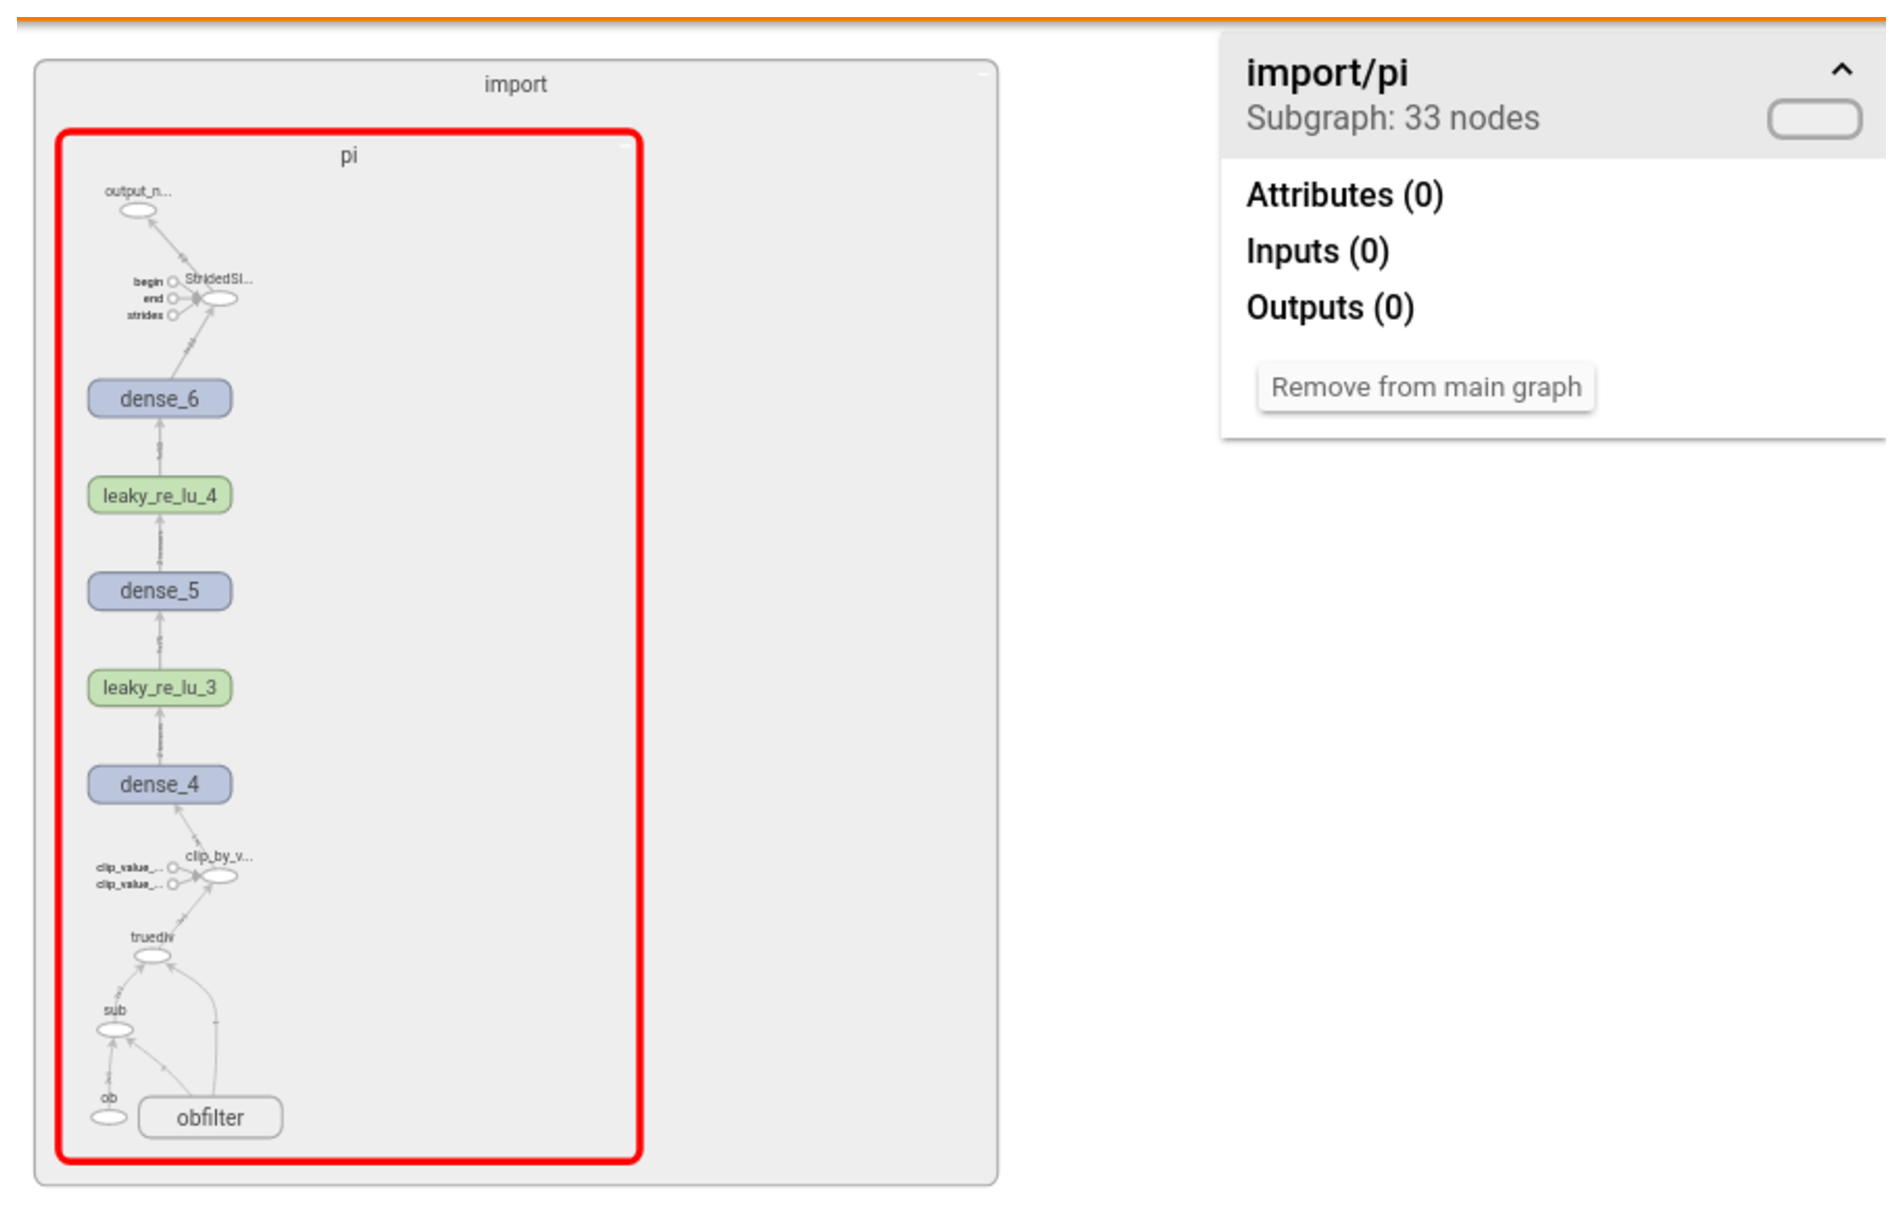
\includegraphics[width=1.1\textwidth]{Cap5/policygraph2.eps}
	\caption{ Policy data flow graph from Figure \ref{fig:model_plot}
	}
	\label{fig:policygraph2}
\end{figure}


\subsection{Distributed Training}
Reinforcement Learning training is much more costly computationally when compared to the supervised one described in \ref{supervised_learning_setup}. Additionally to the costs of applying gradients in the network, we need to gather all the data from agent simulations. Furthermore, since the data distribution changes during the learning, it's harder to converge, se it is needed a large amount of data.

In this context, use a single agent to get all the data and train the algorithm takes too long time to converge and, depending of the problem, it is not viable. We need a way to get more data faster and accelerate the training.

\subsubsection{Data Parallelism}

The solution for this challenge is distribute the training using several agents. Each agent interacts with its own environment, but the results are applied to the same network. This technique is called Data Parallelism, because the parallelization happens in data gathering. It opposes the idea of Model Parallelism, where the learning model itself is distributed, but this technique is not interesting in reinforcement learning training.

In Data Parallelism, we applied a master-workers architecture, as shown in Figure \ref{fig:master-worker}. It has several worker nodes, whose job is gather data by simulating the agent, and a master node, which controls the learning algorithm. This architecture works very well in this experiment because the computation from workers are very similar so we can conduct several independent processes in those. It can also be fault tolerant: if one worker dies, the learning process can keep running.

\begin{figure}[!htbp]
	\centering
	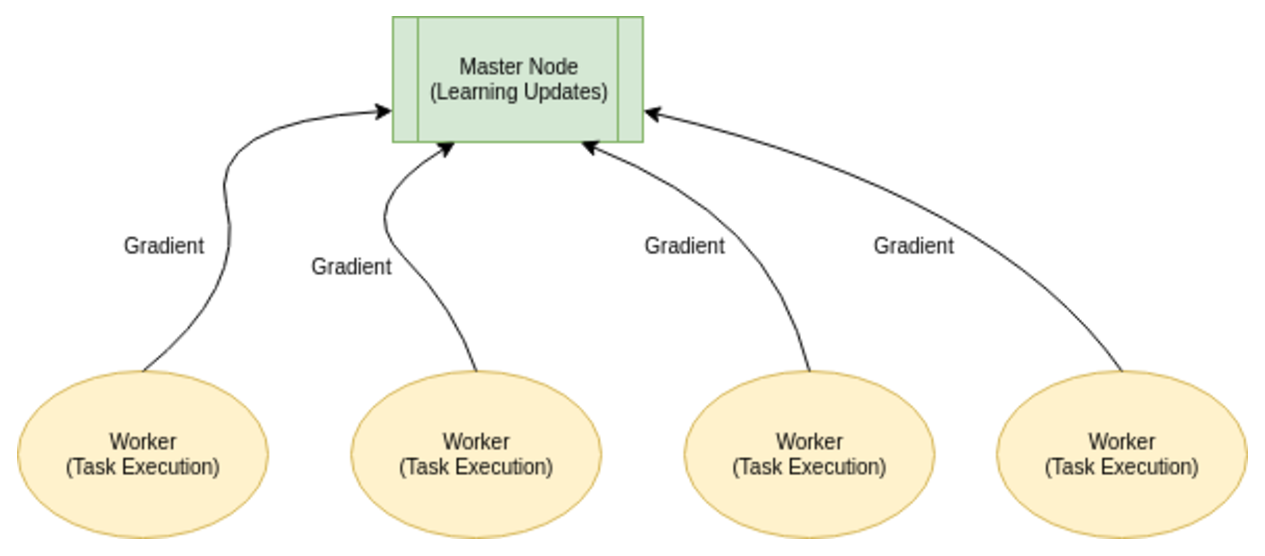
\includegraphics[width=1.1\textwidth]{Cap5/master-worker.eps}
	\caption{ Master-workers architecture for data parallelism.
	}
	\label{fig:master-worker}
\end{figure}

\subsubsection{Synchronous vs. Asynchronous Distributed Training}

There are two ways to apply updates from a master-workers architecture in the learning algorithm. Both ways are illustrated in Figure \ref{fig:distributedtraining}.

In asynchronous training, each worker executes the task, gathers data, calculate the gradient and apply it in the neural network. There's no interaction between workers so the learning updates can occur freely and, therefore, faster. However, the downside is that each worker has its own version of the network which can cause a discrepancy between them and slows the convergence.

On the other side, in the synchronous training, each worker executes the same job as the asynchronous one. However, the master node collects the gradients and applies an average from them. In this way, the updates occurs in the same frequency, but they are much more precise (and therefore we can use large learning rates). 

\cite{heess2017} implemented a variation of PPO called Distributed PPO (DPPO) and their experiments shows that synchronous updates worked better in practice. Hence, in this experimentation we also used this type of distributed training.

\begin{figure}[!htbp]
	\centering
	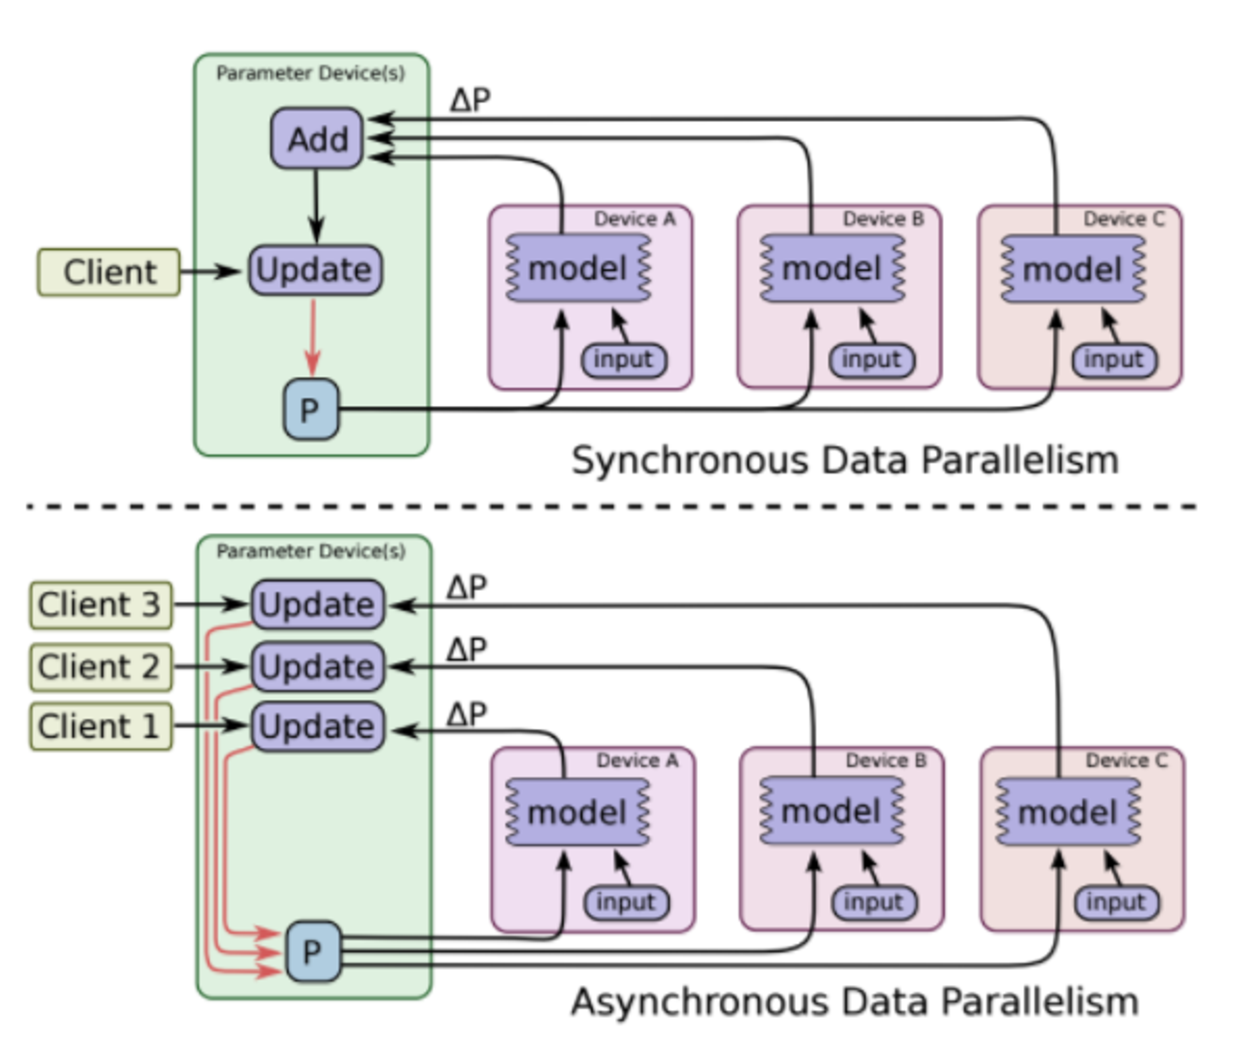
\includegraphics[width=0.8\textwidth]{Cap5/distributedtraining.eps}
	\caption{ Synchronous and Asynchornous Distributed Training.
	}
	\label{fig:distributedtraining}
\end{figure}

\subsection{Metrics}

We need evaluation metrics to compare the techniques in section \ref{sec:experimentation_setup}. Several of them were collected and described below:

\begin{itemize}
	\item \textbf{Episode Reward Mean}: This metric is the mean of cumulate reward during the whole episode. It's directly related to the motion performance. Then, it's the main metric in the comparison.
	\item \textbf{Value Function Loss}: Says how good is the prediction of value function by the network.
	\item \textbf{Timesteps So Far}: It means how many cycles (observation-action-reward) have been executed. This metric was used to compare the speedup from distributed training.
	\item \textbf{Episode Length Mean}: In the case of models with no fixed length, this metric will allow us to understand how the learning worked.
\end{itemize} 

\subsection{Monitoring via Tensorboard}
Lastly, we need a tool whose purpose is monitor the metrics collected during the training. We used Tensorboard \cite{tensorboard}, a graphic visualizer tool from Tensorflow. Figure \ref{fig:tensorboard} shows the GUI with some metrics. Using that, we can compare several models and their metrics, visualize computational graphs and debug the learning process.

\begin{figure}[!htbp]
	\centering
	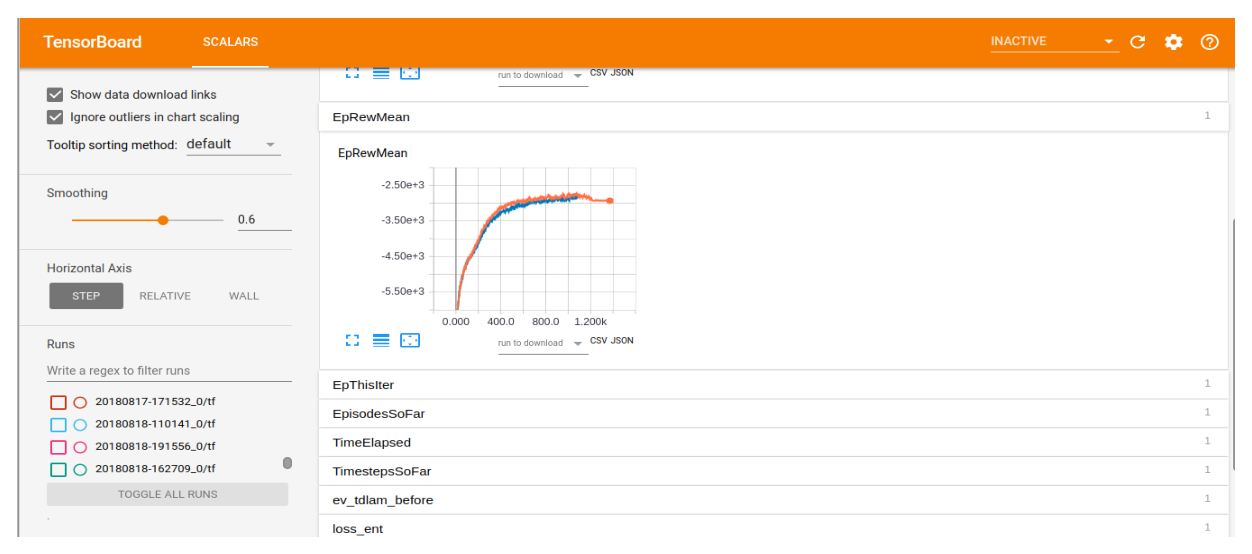
\includegraphics[width=1.0\textwidth]{Cap5/tensorboard.eps}
	\caption{ Monitoring training metrics with Tensorboard.
	}
	\label{fig:tensorboard}
\end{figure}